% udemy_data_course_slides.tex
% Compile with: pdflatex udemy_data_course_slides.tex
\documentclass{beamer}
\usetheme{Madrid}
\usecolortheme{default}

% Packages
\usepackage[utf8]{inputenc}
\usepackage{graphicx}
\usepackage{hyperref}
\usepackage{xcolor}
\usepackage{tikz}
\usepackage{amsmath}

% Smaller fonts for better fit
\setbeamerfont{itemize/enumerate body}{size=\small}
\setbeamerfont{itemize/enumerate subbody}{size=\footnotesize}
\setbeamerfont{block title}{size=\small}
\setbeamerfont{block body}{size=\small}

% Title information
\title{Data Permissions, Sources, Tools, Connections}
\subtitle{Complete Course for Enterprise Data Professionals}
\author{Shivgan Joshi}
\institute{Udemy}
\date{2026}

\begin{document}
	
	% ============================================================
	% TITLE SLIDE
	% ============================================================
	\begin{frame}
		\titlepage
	\end{frame}
	
	% ============================================================
	% SECTION 1: INTRODUCTION (8 slides)
	% ============================================================
	\section{Introduction to Data and Course}
	
	\begin{frame}{Course Overview}
		\begin{block}{What You Will Learn}
			\begin{itemize}
				\item Working with Data at enterprise scale (20-100M+ rows)
				\item Understanding Permissions and data governance
				\item Exploring data sources across different environments
				\item Tools like Toad, Teradata, PySpark, SAS
				\item Connections and troubleshooting real errors
			\end{itemize}
		\end{block}
		\begin{alertblock}{Prerequisite}
			Basic SQL knowledge recommended.
		\end{alertblock}
	\end{frame}
	
	
	\begin{frame}{Course Complete Reference Table}
		\tiny
		\begin{tabular}{|p{0.08\textwidth}|p{0.1\textwidth}|p{0.35\textwidth}|p{0.28\textwidth}|}
			\hline
			\textbf{Sec} & \textbf{Topic} & \textbf{Key Concepts} & \textbf{Tools / Commands} \\
			\hline
			1 & Data Basics & Permissions, Big Data (20-100M rows), Hive tables & SELECT, FROM, WHERE, LIMIT \\
			\hline
			2 & Permissions & PROD/DEV/UAT, Table not found, Confidential levels & Wiki search, Ticketing system \\
			\hline
			3 & ODBC & Manual DSN, Auto connection strings & Driver=\{Teradata\}; DBCName=tdprod \\
			\hline
			3 & Toad & ALT+F+N, Native vs ODBC, New Connection Wizard & Teradata(.NET), Oracle(ODP.NET), Vertica(ODBC only) \\
			\hline
			3 & Auth & Manual, Windows SSO (Teradata/Oracle), Extra Strings & Mechanism, Account String, LDAP, Kerberos \\
			\hline
			4 & Teradata & MPP, Big Data \#1, High cost, EDW & SELECT TOP 100, Primary Index \\
			\hline
			4 & Oracle & OLTP, Shared Everything, Very High cost & PL/SQL, TNS, Wallet \\
			\hline
			4 & Vertica & Columnar, Fast analytics, 64-bit ODBC only & Columnar storage, Projections \\
			\hline
			4 & Hive & Data Lake, Cheap storage, Batch only & HDFS, Parquet, ORC \\
			\hline
			5 & Banking & Teradata=Truth, Vertica=Speed, Hive=Scale & 10yr history, 50M txns/day, 500B archive \\
			\hline
			5 & Joins & INNER, LEFT, RIGHT, FULL, CROSS, SELF, ANTI, SEMI & Venn diagram \\
			\hline
			5 & Optimization & Indexes, Filter early, Avoid SELECT *, EXPLAIN & Partition pruning, LIMIT \\
			\hline
			5 & AI & SQL to PySpark conversion & df.groupBy().sum().show() \\
			\hline
			6 & SAS & Logistic Regression, Regulatory compliance & PROC LOGISTIC, PROC PRINT \\
			\hline
			\multicolumn{4}{|c|}{\textcolor{blue}{Bank Golden Rule: Teradata=Truth $\vert$ Vertica=Speed $\vert$ Hive=Scale}} \\
			\hline
			\multicolumn{4}{|c|}{\textcolor{orange}{Do not join across systems in real-time. Move data to one place first.}} \\
			\hline
		\end{tabular}
		
		\vspace{0.2cm}
		\begin{center}
			\textcolor{green}{\tiny Total: 48 Slides $\vert$ 20+ Lectures $\vert$ Real-life Scenarios}
		\end{center}
	\end{frame}
	
	\begin{frame}{Course Format}
		\begin{example}{Course Structure}
			\begin{itemize}
				\item 20+ Lectures
				\item Real-life Issue Scenarios
				\item Hands-on Examples
				\item Quiz Questions
				\item Practice Exercises
			\end{itemize}
		\end{example}
		\begin{center}
			\textcolor{blue}{Total Slides: 48}
		\end{center}
	\end{frame}
	
	\begin{frame}{Lecture 1: Introduction to Working with Data}
		\begin{definition}{Data Permissions}
			Checking permissions helps understand:
			\begin{itemize}
				\item What the data is about
				\item Who can access it
				\item What operations are allowed
			\end{itemize}
		\end{definition}
		\begin{example}
			Data exists in enterprise at different levels, with different permissions, and in various formats.
		\end{example}
	\end{frame}
	
	\begin{frame}{Lecture 2: Data, Big Data, and Very Big Data}
		\begin{block}{Scale Matters}
			Most of our work will with very big data:
			\begin{itemize}
				\item \textcolor{red}{20 - 100 million data points}
				\item Resides in Hive tables
				\item Accessed through various challenges
			\end{itemize}
		\end{block}
		\begin{center}
			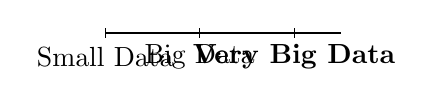
\begin{tikzpicture}[scale=0.6]
				\draw[thick, -] (0,0) -- (5,0);
				\foreach \x in {0,2,4}
				\draw (\x,0.1) -- (\x,-0.1);
				\node at (0,-0.5) {Small Data};
				\node at (2,-0.5) {Big Data};
				\node at (4,-0.5) {\textbf{Very Big Data}};
			\end{tikzpicture}
		\end{center}
	\end{frame}
	
	\begin{frame}{Data Size Comparison Table}
		\begin{table}
			\small
			\begin{tabular}{|l|l|l|}
				\hline
				\textbf{Size Category} & \textbf{Rows} & \textbf{Typical Location} \\
				\hline
				Small & Under 1M & Excel, CSV, Access \\
				\hline
				Big & 1M - 20M & SQL Server, Oracle, MySQL \\
				\hline
				Very Big & 20M - 100M+ & Hive, Teradata, Big Data \\
				\hline
			\end{tabular}
		\end{table}
		\begin{alertblock}{Key Insight}
			Very big data resides in Hive tables but accessed through various challenges.
		\end{alertblock}
	\end{frame}
	
	
	\begin{frame}{Lecture 3: Implementation Team and Framework}
		\begin{block}{How the Implementation Team Works}
			\begin{itemize}
				\item \textbf{Who they are:} Technical team (DBAs, data engineers, platform leads)
				\item \textbf{What they do:} Deploy, schedule, and monitor data models in production
				\item \textbf{Why it's complex:} Models run across different databases (Teradata, Vertica, Hive)
				\item \textbf{Key reality:} Models might need high resources (CPU, memory, I/O)
			\end{itemize}
		\end{block}
		
		\begin{alertblock}{Framework in Action}
			\begin{enumerate}
				\small
				\item Business defines model logic
				\item Implementation team translates to SQL / PySpark / SAS
				\item Team requests permissions and connections
				\item Execution happens in batch or near-real-time
				\item Team monitors performance and troubleshoots errors
			\end{enumerate}
		\end{alertblock}
		
		\begin{example}{Real-World Complexity}
			A single customer risk model may:
			\begin{itemize}
				\tiny
				\item Pull from Teradata (master data)
				\item Join with Vertica (recent transactions)
				\item Enrich with Hive (historical patterns)
				\item Run in SAS (regression)
				\item Fail if any connection, permission, or resource is missing
			\end{itemize}
		\end{example}
		
		\begin{center}
			\textcolor{orange}{Implementation is not just code — it's orchestration, resources, and troubleshooting.}
		\end{center}
	\end{frame}
	
	\begin{frame}{Lecture 3: Implementation Team and Framework}
		\begin{itemize}
			\item Implementation is a complex phenomenon
			\item The implementation team:
			\begin{itemize}
				\item Runs the models
				\item Requires high resources
				\item Manages technical infrastructure
			\end{itemize}
		\end{itemize}
		\begin{quote}
			Models might need high resources - plan ahead!
		\end{quote}
	\end{frame}
	
	\begin{frame}{Lecture 4: How to Run a Query or Request Data}
		\begin{enumerate}
			\item Connect to the database (ODBC or Native)
			\item Check your permissions
			\item Write your query (SELECT, FROM, WHERE)
			\item Execute and fetch results
			\item Handle errors if any
		\end{enumerate}
		\vspace{0.3cm}
		\textbf{Example Query:}
		\begin{center}
			\color{blue}
			SELECT * FROM employee\_data \\
			WHERE department = SALES \\
			LIMIT 100;
			\color{black}
		\end{center}
	\end{frame}
	
	\begin{frame}{Where Data Resides in Enterprise}
		\begin{center}
			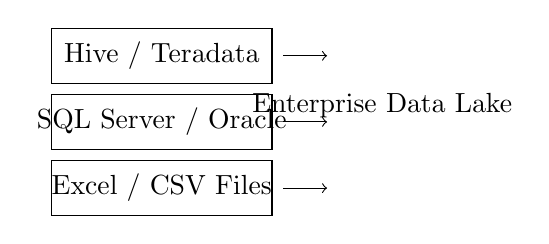
\begin{tikzpicture}[scale=0.7]
				\draw (0,0) rectangle (4,1);
				\node at (2,0.5) {Excel / CSV Files};
				\draw (0,1.2) rectangle (4,2.2);
				\node at (2,1.7) {SQL Server / Oracle};
				\draw (0,2.4) rectangle (4,3.4);
				\node at (2,2.9) {Hive / Teradata};
				\draw[->] (4.2,0.5) -- (5,0.5);
				\draw[->] (4.2,1.7) -- (5,1.7);
				\draw[->] (4.2,2.9) -- (5,2.9);
				\node at (6,2) {Enterprise Data Lake};
			\end{tikzpicture}
		\end{center}
	\end{frame}
	
	% ============================================================
	% SECTION 2: PERMISSIONS (6 slides)
	% ============================================================
	\section{Permissions for Tools and Databases}
	
	\begin{frame}{Lecture 5: Raising Permissions Steps}
		\begin{block}{Permission Request Process}
			\begin{enumerate}
				\item You get a new error (access denied, table not found)
				\item Search for Notes or Wiki about the permission
				\item Identify the required permission level
				\item Submit a request via ticketing system
			\end{enumerate}
		\end{block}
		\begin{example}
			Example: You have PROD and DEV permission, but not UAT permission.
		\end{example}
	\end{frame}
	
	\begin{frame}{Lecture 6: Permission Errors}
		\begin{alertblock}{Common Permission Errors}
			\begin{itemize}
				\item \textbf{Table not found} - (You don't have SELECT permission)
				\item \textbf{Database not found} - (No access to the schema)
				\item \textbf{Server connection refused} - (Network or firewall)
				\item \textbf{ODBC driver error} - (Driver not installed or configured)
			\end{itemize}
		\end{alertblock}
	\end{frame}
	
	\begin{frame}{Permission Error Resolution Matrix}
		\begin{table}
			\small
			\begin{tabular}{|p{0.35\textwidth}|p{0.55\textwidth}|}
				\hline
				\textbf{Error Message} & \textbf{Solution} \\
				\hline
				Table not found & Request SELECT permission from DBA \\
				\hline
				Database not found & Request schema access \\
				\hline
				Access denied & Check role or group membership \\
				\hline
				View not found & Missing underlying table access \\
				\hline
			\end{tabular}
		\end{table}
	\end{frame}
	
	\begin{frame}{Lecture 7: Confidential vs Very Confidential Permission}
		\begin{columns}[T]
			\column{0.48\textwidth}
			\begin{block}{Normal Permission}
				\begin{itemize}
					\item PII data
					\item Financial records
					\item Internal reports
					\item Accessible by many teams
				\end{itemize}
			\end{block}
			
			\column{0.48\textwidth}
			\begin{alertblock}{Very Confidential}
				\begin{itemize}
					\item Trade secrets
					\item Executive data
					\item Merger info
					\item Needs special approval
				\end{itemize}
			\end{alertblock}
		\end{columns}
	\end{frame}
	
	\begin{frame}{Permission Levels by Data Type}
		\begin{center}
			\begin{tabular}{|l|c|c|}
				\hline
				\textbf{Data Type} & \textbf{Permission Level} & \textbf{Approval} \\
				\hline
				Public Data & Low & Self-service \\
				\hline
				Internal Reports & Medium & Manager \\
				\hline
				PII / PHI & High & Compliance \\
				\hline
				Trade Secrets & Very High & Executive \\
				\hline
			\end{tabular}
		\end{center}
	\end{frame}
	
	\begin{frame}{Best Practices for Permissions}
		\begin{block}{Security Best Practices}
			\begin{itemize}
				\item Least privilege principle
				\item Regular permission audits
				\item Use groups instead of individual grants
				\item Document all permission requests
				\item Set expiration for temporary access
			\end{itemize}
		\end{block}
		\begin{center}
			\textcolor{orange}{Always verify permission level before accessing sensitive data!}
		\end{center}
	\end{frame}
	
	% ============================================================
	% SECTION 3: CONNECTIONS (10 slides)
	% ============================================================
	\section{Connections - ODBC, Native, Authentication}
	
	\begin{frame}{Lecture 8: Connection through ODBC}
		\begin{definition}{ODBC}
			Open Database Connectivity - Standard API for accessing database management systems.
		\end{definition}
		\begin{itemize}
			\item \textbf{Manual ODBC}: Configure DSN manually in Control Panel
			\item \textbf{Automatic ODBC}: Connection strings or application config
		\end{itemize}
	\end{frame}
	
	\begin{frame}{ODBC Connection String Examples}
		\textbf{Teradata Example:}
		\begin{center}
			\color{blue}
			Driver=\{Teradata\};DBCName=tdprod;\\
			Database=my\_db;UID=user;PWD=pass;
			\color{black}
		\end{center}
		
		\textbf{Oracle Example:}
		\begin{center}
			\color{blue}
			Driver=\{Oracle in OraClient\};\\
			Data Source=ORCL;UID=user;PWD=pass;
			\color{black}
		\end{center}
	\end{frame}
	
	\begin{frame}{Lecture 9: Connections at TOAD}
		\begin{block}{TOAD Connection Screens}
			\begin{itemize}
				\item \textbf{New Connection Wizard}
				\item Connection Type selection (Oracle, SQL Server, Teradata)
				\item Authentication method (Windows, LDAP, Database)
				\item Advanced settings (SSL, Proxy)
			\end{itemize}
		\end{block}
		\begin{center}
			\textcolor{blue}{Shortcut:} ALT+F+N
		\end{center}
	\end{frame}
	
	\begin{frame}{Toad Connection Methods: Native vs ODBC}
		\begin{table}
			\small
			\begin{tabular}{|l|c|c|c|}
				\hline
				\textbf{Feature} & \textbf{Teradata} & \textbf{Oracle} & \textbf{Vertica} \\
				\hline
				Native Driver & .NET Provider & ODP.NET & \textcolor{red}{None} \\
				\hline
				ODBC Support & Yes & Yes & \textcolor{green}{Only} \\
				\hline
				Windows SSO & Yes & Yes & \textcolor{red}{No} \\
				\hline
				LDAP Support & Yes & Yes & \textcolor{red}{No} \\
				\hline
				\textbf{Recommended} & \textbf{Native} & \textbf{Native} & \textbf{ODBC} \\
				\hline
			\end{tabular}
		\end{table}
	\end{frame}
	
	\begin{frame}{Vertica ODBC Requirements}
		\begin{alertblock}{Critical: Bitness Mismatch}
			\begin{itemize}
				\item Toad 2025 R2+ is 64-bit only
				\item Must use 64-bit Vertica ODBC driver
				\item 32-bit driver will fail to connect
			\end{itemize}
		\end{alertblock}
		\begin{example}{Solution}
			Download and install 64-bit Vertica ODBC driver from vendor website.
		\end{example}
	\end{frame}
	
	\begin{frame}{Authentication Methods Comparison}
		\begin{columns}[T]
			\column{0.32\textwidth}
			\begin{block}{Manual}
				\begin{itemize}
					\small
					\item Type user/password
					\item Works for ALL
					\item Most common
				\end{itemize}
			\end{block}
			
			\column{0.32\textwidth}
			\begin{block}{Windows SSO}
				\begin{itemize}
					\small
					\item Uses Windows login
					\item No password typing
					\item \textcolor{red}{Not for Vertica}
				\end{itemize}
			\end{block}
			
			\column{0.32\textwidth}
			\begin{block}{Extra Strings}
				\begin{itemize}
					\small
					\item Mechanism
					\item Account String
					\item LDAP or Kerberos
				\end{itemize}
			\end{block}
		\end{columns}
	\end{frame}
	
	\begin{frame}{Database Authentication by Type}
		\begin{center}
			\begin{tabular}{|l|c|c|c|}
				\hline
				\textbf{Database} & \textbf{Manual} & \textbf{Windows SSO} & \textbf{Extra Strings} \\
				\hline
				Teradata & Yes & Yes & Mechanism, Account \\
				\hline
				Oracle & Yes & Yes & TNS, LDAP, Wallet \\
				\hline
				Vertica & Yes & \textcolor{red}{No} & DSN Parameters \\
				\hline
				SQL Server & Yes & Yes & None needed \\
				\hline
				MySQL & Yes & No & None needed \\
				\hline
			\end{tabular}
		\end{center}
	\end{frame}
	
\begin{frame}{Lecture 10: Different Kinds of Databases}
	\begin{table}
		\small
		\begin{tabular}{|l|l|}
			\hline
			\textbf{Database Type} & \textbf{Examples} \\
			\hline
			Relational & Oracle, MySQL, SQL Server, PostgreSQL \\
			\hline
			MPP / Data Warehouse & Teradata, Redshift, Snowflake, \textcolor{blue}{Vertica} \\
			\hline
			Hadoop / Big Data & Hive, HBase, Spark SQL \\
			\hline
			NoSQL & MongoDB, Cassandra \\
			\hline
			Columnar & ClickHouse (Vertica listed above as MPP) \\
			\hline
		\end{tabular}
	\end{table}
	
	\vspace{0.3cm}
	\begin{center}
		\textcolor{blue}{\tiny Note: Vertica is both MPP and Columnar – best of both worlds}
	\end{center}
\end{frame}
	
	

\begin{frame}{Bank Transaction Data: Teradata vs Vertica}
	\tiny
	\begin{center}
		\begin{tabular}{|p{0.05\textwidth}|p{0.43\textwidth}|p{0.43\textwidth}|}
			\hline
			& \textcolor{blue}{\textbf{Teradata}} & \textcolor{green}{\textbf{Vertica}} \\
			\hline
			\textbf{Role} & System of Record & Analytics Engine \\
			\hline
			\textbf{Kind of Data} & Final, cleansed, audited, official & Processed, aggregated, enriched \\
			\hline
			\textbf{Data Examples} & Daily balances, official ledgers, audit trails & Fraud scores, real-time alerts, dashboards \\
			\hline
			\textbf{Data Size} & 10+ years (500B+ rows, PB scale) & 30-90 days (50M-1B rows) \\
			\hline
			\textbf{Query Speed} & Complex joins: 5-10 min & Aggregations: 20-50 ms \\
			\hline
			\textbf{Load Speed} & Very fast (bulk load) & Fast (columnar insert) \\
			\hline
			\textbf{Concurrency} & High (1000+ users) & Medium (100+ users) \\
			\hline
			\textbf{Example Query} & "Official balance for account 12345 as of Dec 31, 2023" & "Flag transactions over \$10k from new locations in last 5 min" \\
			\hline
			\textbf{Best For} & Regulatory reports, end-of-day, audits & Real-time fraud, live dashboards, ad-hoc analytics \\
			\hline
		\end{tabular}
	\end{center}
	
	\vspace{0.15cm}
	\begin{center}
		\textcolor{orange}{\scriptsize Real Bank: 50M transactions/day → Teradata (night) → Vertica (morning for fast queries)}
	\end{center}
\end{frame}



	\begin{frame}{HDFS / Hadoop (Data Lake)}
		\begin{block}{\textcolor{orange}{What It Is}}
			\begin{itemize}
				\tiny
				\item \textbf{Type:} Distributed file system
				\item \textbf{Stores:} Raw files (CSV, JSON, logs)
				\item \textbf{Processing:} Spark, MapReduce
				\item \textbf{Schema:} On-read (flexible)
			\end{itemize}
		\end{block}
		
		\begin{center}
			\textcolor{orange}{\tiny "Dump everything here first, process later"}
		\end{center}
		
		\begin{example}{Examples}
			\tiny
			HDFS, Apache Hadoop, Azure Data Lake Storage, Amazon S3
		\end{example}
		
		\begin{table}
			\tiny
			\begin{tabular}{|p{0.3\textwidth}|p{0.6\textwidth}|}
				\hline
				\textbf{Best For} & Raw data storage, data lakes, big raw data \\
				\hline
				\textbf{Who Uses It} & Data engineers \\
				\hline
				\textbf{Query Speed} & Slower (needs Spark engine) \\
				\hline
			\end{tabular}
		\end{table}
		
		\begin{center}
			\textcolor{blue}{\tiny Think: Storage first, process later}
		\end{center}
	\end{frame}
	
	
	\begin{frame}{Data Flow: Data Lake → Data Warehouse}
		\begin{center}
			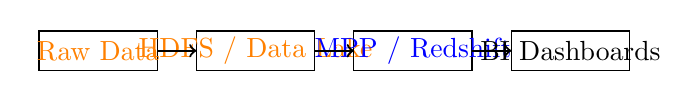
\begin{tikzpicture}[scale=0.5]
				\draw (0,0) rectangle (3,1);
				\node at (1.5,0.5) {\textcolor{orange}{Raw Data}};
				
				\draw (4,0) rectangle (7,1);
				\node at (5.5,0.5) {\textcolor{orange}{HDFS / Data Lake}};
				
				\draw (8,0) rectangle (11,1);
				\node at (9.5,0.5) {\textcolor{blue}{MPP / Redshift}};
				
				\draw (12,0) rectangle (15,1);
				\node at (13.5,0.5) {BI Dashboards};
				
				\draw[->, thick] (3,0.5) -- (4,0.5);
				\draw[->, thick] (7,0.5) -- (8,0.5);
				\draw[->, thick] (11,0.5) -- (12,0.5);
			\end{tikzpicture}
		\end{center}
		
		\begin{center}
			\tiny
			Raw Data → Data Lake (HDFS) → ETL/ELT → Data Warehouse (MPP) → Dashboards
		\end{center}
		
		\begin{alertblock}{Quick Takeaway}
			\tiny
			\textcolor{orange}{HDFS} stores raw data. \textcolor{blue}{MPP (Redshift)} analyzes cleaned data very fast using SQL.
		\end{alertblock}
	\end{frame}
	
	\begin{frame}{Lecture 11: Connection Errors}
		\begin{alertblock}{Common Connection Errors}
			\begin{itemize}
				\item \textbf{Timeout} - Server not responding
				\item \textbf{Authentication failed} - Wrong credentials
				\item \textbf{Driver not found} - Missing ODBC or JDBC driver
				\item \textbf{Network unreachable} - VPN or Firewall issues
				\item \textbf{Maximum connections reached} - Too many users
			\end{itemize}
		\end{alertblock}
	\end{frame}
	
	\begin{frame}{Real-Life Connection Issues from Toad World}
		\begin{columns}[T]
			\column{0.48\textwidth}
			\begin{alertblock}{Issue \#1: No Teradata Option}
				\textbf{Problem:} TDA 2.6 no Teradata in Group
				\begin{itemize}
					\item Root cause: Version too old
					\item .NET support added in 3.x
					\item Solution: Upgrade to 3.x or use ODBC
				\end{itemize}
			\end{alertblock}
			
			\column{0.48\textwidth}
			\begin{alertblock}{Issue \#2: Timeout Error}
				\textbf{Problem:} Command did not complete within timeout
				\begin{itemize}
					\item Root cause: Long query
					\item Solution: Increase timeout or optimize query
				\end{itemize}
			\end{alertblock}
		\end{columns}
	\end{frame}
	
	% ============================================================
	% SECTION 4: DATABASE COMPARISON (8 slides)
	% ============================================================
	\section{Teradata vs Oracle vs Vertica}
	
	\begin{frame}{Why Three Different Databases?}
		\begin{center}
			\begin{tabular}{|p{0.3\textwidth}|p{0.3\textwidth}|p{0.3\textwidth}|}
				\hline
				\textcolor{blue}{\textbf{Teradata}} & \textcolor{orange}{\textbf{Oracle}} & \textcolor{green}{\textbf{Vertica}} \\
				\hline
				MPP Data Warehouse & OLTP + Warehouse & Columnar Analytics \\
				\hline
				Big Data (PB scale) & Mixed Workload & Fast Analytics \\
				\hline
				High Cost & Very High Cost & Moderate Cost \\
				\hline
				Best for EDW & Best for Transactions & Best for Reporting \\
				\hline
			\end{tabular}
		\end{center}
		\begin{quote}
			No single database fits all needs - choose based on your workload!
		\end{quote}
	\end{frame}
	
	\begin{frame}{Feature Comparison: Architecture}
		\begin{table}
			\small
			\begin{tabular}{|p{0.3\textwidth}|c|c|c|}
				\hline
				\textbf{Feature} & \textbf{Teradata} & \textbf{Oracle} & \textbf{Vertica} \\
				\hline
				Architecture & MPP Shared Nothing & Shared Everything & Columnar MPP \\
				\hline
				Storage Type & Row-based & Row-based & Columnar \\
				\hline
				Indexing & Primary Index & B-Tree, Bitmap & Projections \\
				\hline
				Compression & Moderate & Good & Excellent \\
				\hline
			\end{tabular}
		\end{table}
	\end{frame}
	
	\begin{frame}{Feature Comparison: Performance}
		\begin{table}
			\small
			\begin{tabular}{|p{0.3\textwidth}|c|c|c|}
				\hline
				\textbf{Performance} & \textbf{Teradata} & \textbf{Oracle} & \textbf{Vertica} \\
				\hline
				Big Data Ready & Best & Needs Exadata & Good \\
				\hline
				Analytics Speed & Fast & Fast (indexed) & Very Fast \\
				\hline
				Load Speed & Very Fast & Moderate & Fast \\
				\hline
				Query Concurrency & High & Very High & Medium \\
				\hline
			\end{tabular}
		\end{table}
	\end{frame}
	
	\begin{frame}{Which One is FASTEST?}
		\begin{columns}[T]
			\column{0.5\textwidth}
			\textbf{For Big Data (Billions of rows):}
			\begin{itemize}
				\item \textcolor{blue}{Teradata} \#1 - MPP architecture
				\item Vertica - Very fast for analytics
				\item Oracle - Needs tuning for big data
			\end{itemize}
			
			\vspace{0.3cm}
			\textbf{For Speed (Queries under 1 second):}
			\begin{itemize}
				\item \textcolor{green}{Vertica} - Columnar storage
				\item Oracle - With proper indexes
				\item Teradata - Good for complex queries
			\end{itemize}
			
			\column{0.5\textwidth}
			\textbf{Which Has Big Data Built-in?}
			\begin{itemize}
				\item \textcolor{blue}{Teradata} - Designed for PB scale
				\item Vertica - Scales well
				\item Oracle - Needs Exadata for big data
			\end{itemize}
		\end{columns}
	\end{frame}
	
	\begin{frame}{Detailed Comparison Table}
		\begin{table}
			\tiny
			\begin{tabular}{|p{0.22\textwidth}|p{0.24\textwidth}|p{0.24\textwidth}|p{0.24\textwidth}|}
				\hline
				\textbf{Feature} & \textbf{Teradata} & \textbf{Vertica} & \textbf{Oracle} \\
				\hline
				Architecture & MPP Shared Nothing & Columnar MPP & Shared Everything \\
				\hline
				Best For & EDW, Big Data & Analytics, Reporting & OLTP, Mixed Workload \\
				\hline
				Compression & Moderate & Excellent & Good \\
				\hline
				Load Speed & Very Fast & Fast & Moderate \\
				\hline
				Query Speed (Analytics) & Fast & Very Fast & Fast with indexes \\
				\hline
				Cost & High & Moderate & Very High \\
				\hline
				Cloud Ready & Yes (Vantage) & Yes & Yes (OCI) \\
				\hline
			\end{tabular}
		\end{table}
	\end{frame}
	
	\begin{frame}{Use Case: When to Use Which?}
		\begin{columns}[T]
			\column{0.33\textwidth}
			\begin{block}{\textcolor{blue}{Teradata}}
				\begin{itemize}
					\small
					\item Billions+ rows
					\item Enterprise Data Warehouse
					\item Complex joins on large tables
					\item Regulatory compliance needed
				\end{itemize}
			\end{block}
			
			\column{0.33\textwidth}
			\begin{block}{\textcolor{green}{Vertica}}
				\begin{itemize}
					\small
					\item Fast analytics on large data
					\item Time-series analysis
					\item Log data analysis
					\item Lower cost than Teradata
				\end{itemize}
			\end{block}
			
			\column{0.33\textwidth}
			\begin{block}{\textcolor{orange}{Oracle}}
				\begin{itemize}
					\small
					\item OLTP (many writes)
					\item Existing Oracle ecosystem
					\item Mixed workloads
					\item Need PL/SQL
				\end{itemize}
			\end{block}
		\end{columns}
	\end{frame}
	
	\begin{frame}{Industry-Specific Recommendations}
		\begin{columns}[T]
			\column{0.33\textwidth}
			\textbf{Banking/Finance}
			\begin{itemize}
				\small
				\item Teradata - Risk analysis
				\item Oracle - Core banking
				\item Vertica - Fraud detection
			\end{itemize}
			
			\column{0.33\textwidth}
			\textbf{Retail/Ecommerce}
			\begin{itemize}
				\small
				\item Teradata - Customer 360
				\item Vertica - Real-time analytics
				\item Oracle - Order processing
			\end{itemize}
			
			\column{0.33\textwidth}
			\textbf{Healthcare}
			\begin{itemize}
				\small
				\item Oracle - Patient records
				\item Teradata - Population health
				\item Vertica - Research analytics
			\end{itemize}
		\end{columns}
	\end{frame}
	
	\begin{frame}{Quick Decision Guide}
		\begin{center}
			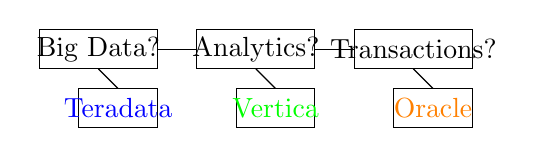
\begin{tikzpicture}[scale=0.5]
				\draw (0,2) rectangle (3,3);
				\node at (1.5,2.5) {Big Data?};
				\draw (4,2) rectangle (7,3);
				\node at (5.5,2.5) {Analytics?};
				\draw (8,2) rectangle (11,3);
				\node at (9.5,2.5) {Transactions?};
				
				\draw[-] (3,2.5) -- (4,2.5);
				\draw[-] (7,2.5) -- (8,2.5);
				
				\draw (1,0.5) rectangle (3,1.5);
				\node at (2,1) {\textcolor{blue}{Teradata}};
				\draw (5,0.5) rectangle (7,1.5);
				\node at (6,1) {\textcolor{green}{Vertica}};
				\draw (9,0.5) rectangle (11,1.5);
				\node at (10,1) {\textcolor{orange}{Oracle}};
				
				\draw[-] (1.5,2) -- (2,1.5);
				\draw[-] (5.5,2) -- (6,1.5);
				\draw[-] (9.5,2) -- (10,1.5);
			\end{tikzpicture}
		\end{center}
		\begin{block}{Simple Rule}
			\begin{itemize}
				\item \textcolor{blue}{Teradata} = Enterprise Big Data Warehouse
				\item \textcolor{green}{Vertica} = Fast Columnar Analytics
				\item \textcolor{orange}{Oracle} = Traditional Transactional Database
			\end{itemize}
		\end{block}
	\end{frame}
	
	
	\begin{frame}{Banking Industry: Which Data Goes Where?}
		\begin{center}
			\textcolor{blue}{\Large Real Bank Data Distribution Example}
		\end{center}
		
		\begin{table}
			\small
			\begin{tabular}{|p{0.25\textwidth}|p{0.23\textwidth}|p{0.23\textwidth}|p{0.23\textwidth}|}
				\hline
				\textbf{Data Type} & \textbf{Teradata} & \textbf{Vertica} & \textbf{Hive} \\
				\hline
				Transaction History (10+ years) & \textcolor{blue}{Primary} & Backup & Archive \\
				\hline
				Customer Master Records & \textcolor{blue}{Primary} & Copy & Copy \\
				\hline
				Fraud Detection Alerts & Real-time & \textcolor{green}{Fast Analytics} & Batch \\
				\hline
				Risk Reports (Daily) & Yes & \textcolor{green}{Best} & No \\
				\hline
				Regulatory Filings & Source & Analytics & Staging \\
				\hline
			\end{tabular}
		\end{table}
		
		\begin{alertblock}{Bank's Typical Setup}
			\textbf{Teradata} = System of Record (Gold Source) \\
			\textbf{Vertica} = Fast Analytics and Reporting \\
			\textbf{Hive} = Data Lake and Archival Storage
		\end{alertblock}
	\end{frame}
	
	
	\begin{frame}{Which Data is BIG? Which is FAST?}
		\begin{columns}[T]
			\column{0.5\textwidth}
			\begin{block}{\textcolor{blue}{Big Data (Volume)}}
				\textbf{Teradata and Hive handle:}
				\begin{itemize}
					\small
					\item 10+ years transaction history
					\item Billions of rows per table
					\item PB scale data warehouses
					\item Full customer lifecycle data
				\end{itemize}
			\end{block}
			
			\column{0.5\textwidth}
			\begin{block}{\textcolor{green}{Fast Data (Speed)}}
				\textbf{Vertica excels at:}
				\begin{itemize}
					\small
					\item Fraud detection (seconds)
					\item Real-time risk scoring
					\item Daily P\&L reports
					\item Customer 360 analytics
				\end{itemize}
			\end{block}
		\end{columns}
		
		\begin{center}
			\textcolor{orange}{Teradata = Big and Safe \quad Vertica = Fast and Smart \quad Hive = Cheap and Deep}
		\end{center}
	\end{frame}
	
	
	\begin{frame}{Bank Example: Daily Data Flow}
		\begin{center}
			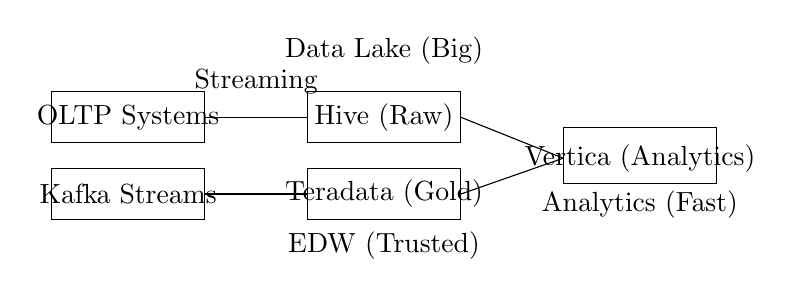
\begin{tikzpicture}[scale=0.65]
				\draw (0,2) rectangle (3,3);
				\node at (1.5,2.5) {OLTP Systems};
				\draw (0,0.5) rectangle (3,1.5);
				\node at (1.5,1) {Kafka Streams};
				
				\draw (5,2) rectangle (8,3);
				\node at (6.5,2.5) {Hive (Raw)};
				\draw (5,0.5) rectangle (8,1.5);
				\node at (6.5,1) {Teradata (Gold)};
				
				\draw (10,1.2) rectangle (13,2.3);
				\node at (11.5,1.7) {Vertica (Analytics)};
				
				\draw[-] (3,2.5) -- (5,2.5);
				\draw[-] (3,1) -- (5,1);
				\draw[-] (8,2.5) -- (10,1.7);
				\draw[-] (8,1) -- (10,1.7);
				
				\node at (4,3.2) {Streaming};
				\node at (6.5,3.8) {Data Lake (Big)};
				\node at (6.5,0) {EDW (Trusted)};
				\node at (11.5,0.8) {Analytics (Fast)};
			\end{tikzpicture}
		\end{center}
		
		\begin{example}{Daily Volume}
			10M transactions → Hive (raw) → Teradata (cleansed) → Vertica (aggregated)
		\end{example}
	\end{frame}
	
	
	\begin{frame}{Bank Use Case: Fraud Detection}
		\begin{columns}[T]
			\column{0.48\textwidth}
			\begin{block}{\textcolor{red}{The Problem}}
				\small
				Bank needs to detect fraudulent transactions in REAL-TIME
				\begin{itemize}
					\item 50,000 transactions per second
					\item Must flag within 100ms
					\item Historical pattern matching needed
				\end{itemize}
			\end{block}
			
			\column{0.48\textwidth}
			\begin{block}{\textcolor{green}{The Solution}}
				\begin{itemize}
					\item \textbf{Vertica} - Real-time scoring engine
					\item \textbf{Teradata} - Historical patterns (last 5 years)
					\item \textbf{Hive} - Long-term archive (10+ years)
				\end{itemize}
			\end{block}
		\end{columns}
		
		\begin{table}
			\small
			\begin{tabular}{|l|c|c|c|}
				\hline
				\textbf{Query Type} & \textbf{Teradata} & \textbf{Vertica} & \textbf{Hive} \\
				\hline
				Real-time fraud check & 50ms & \textcolor{green}{20ms} & 2000ms \\
				\hline
				Daily fraud report & 5 min & \textcolor{green}{2 min} & 15 min \\
				\hline
				Yearly trend analysis & 2 hours & 30 min & \textcolor{green}{20 min} \\
				\hline
			\end{tabular}
		\end{table}
	\end{frame}
	
	
	\begin{frame}{Bank Data Volume Comparison (Actual Numbers)}
		\begin{center}
			\begin{tabular}{|l|c|c|c|}
				\hline
				\textbf{Data Type} & \textbf{Volume} & \textbf{Which DB?} & \textbf{Why?} \\
				\hline
				Daily Transactions & 50M rows & Vertica & Fast queries \\
				\hline
				Monthly Aggregates & 1.5B rows & Teradata & Reliable EDW \\
				\hline
				Historical Archive & 500B rows & Hive & Low cost \\
				\hline
				Customer Profiles & 10M rows & Teradata & ACID compliance \\
				\hline
				Fraud Patterns & 100M rows & Vertica & Columnar speed \\
				\hline
			\end{tabular}
		\end{center}
		
		\begin{alertblock}{Storage Cost Comparison (per TB)}
			Teradata: \$5000/month \quad Vertica: \$1500/month \quad Hive: \$200/month
		\end{alertblock}
	\end{frame}
	
	
	\begin{frame}{Bank: Which Database Wins?}
		\begin{columns}[T]
			\column{0.33\textwidth}
			\begin{block}{\textcolor{blue}{Teradata}}
				\textbf{Wins when:}
				\begin{itemize}
					\small
					\item Data must be 100\% accurate
					\item Complex joins needed
					\item Regulatory reporting
					\item System of record
				\end{itemize}
				\vspace{0.2cm}
				\textcolor{blue}{Example: End-of-day balances}
			\end{block}
			
			\column{0.33\textwidth}
			\begin{block}{\textcolor{green}{Vertica}}
				\textbf{Wins when:}
				\begin{itemize}
					\small
					\item Speed is critical
					\item Aggregations needed
					\item Time-series analysis
					\item Interactive dashboards
				\end{itemize}
				\vspace{0.2cm}
				\textcolor{green}{Example: Real-time fraud detection}
			\end{block}
			
			\column{0.33\textwidth}
			\begin{block}{\textcolor{orange}{Hive}}
				\textbf{Wins when:}
				\begin{itemize}
					\small
					\item Cost is priority
					\item Batch processing OK
					\item Historical analysis
					\item Data lake storage
				\end{itemize}
				\vspace{0.2cm}
				\textcolor{orange}{Example: 10-year audit archive}
			\end{block}
		\end{columns}
	\end{frame}
	
	
	\begin{frame}{Summary: Big vs Fast vs Cheap}
		\begin{center}
			\begin{tabular}{|l|c|c|c|}
				\hline
				& \textbf{Teradata} & \textbf{Vertica} & \textbf{Hive} \\
				\hline
				\textbf{Big Data?} & \checkmark & \checkmark & \checkmark\checkmark \\
				\hline
				\textbf{Fast Queries?} & \checkmark & \checkmark\checkmark & X \\
				\hline
				\textbf{Real-time?} & Moderate & \textcolor{green}{Yes} & No \\
				\hline
				\textbf{Cheap Storage?} & No & No & \textcolor{green}{Yes} \\
				\hline
				\textbf{ACID Transactions?} & \checkmark & X & X \\
				\hline
				\textbf{Best For...} & Gold Source & Analytics & Archive \\
				\hline
			\end{tabular}
		\end{center}
		
		\begin{block}{Bank's Golden Rule}
			\textcolor{blue}{Teradata} = Truth (Single Source of Truth) \\
			\textcolor{green}{Vertica} = Speed (Real-time Analytics) \\
			\textcolor{orange}{Hive} = Scale (Cheap Historical Storage)
		\end{block}
	\end{frame}
	
	
	% ============================================================
	% SECTION 5: QUERIES (6 slides)
	% ============================================================
	\section{Queries - Optimization and AI}
	
	\begin{frame}{Lecture 15: Idea Behind Queries}
		\begin{block}{The Reality}
			\begin{quote}
				Queries are long and hard to understand
			\end{quote}
		\end{block}
		\begin{itemize}
			\item Production queries can be 1000+ lines
			\item Multiple subqueries and CTEs
			\item Complex business logic
			\item Performance tuning required
		\end{itemize}
	\end{frame}
	
	\begin{frame}{Lecture 16: Using Copilot Carefully}
		\begin{alertblock}{AI for Query Conversion}
			\textbf{Converting SQL to PySpark}
		\end{alertblock}
		
		\textbf{SQL:}
		\begin{center}
			\color{blue}
			SELECT col1, SUM(col2) FROM table GROUP BY col1;
			\color{black}
		\end{center}
		
		\textbf{PySpark Equivalent:}
		\begin{center}
			\color{blue}
			df.groupBy("col1").sum("col2").show()
			\color{black}
		\end{center}
		
		\begin{center}
			\textcolor{orange}{Caution: Always validate AI-generated code!}
		\end{center}
	\end{frame}
	
	\begin{frame}{SQL to PySpark Conversion Examples}
		\begin{table}
			\small
			\begin{tabular}{|p{0.45\textwidth}|p{0.45\textwidth}|}
				\hline
				\textbf{SQL} & \textbf{PySpark} \\
				\hline
				SELECT * FROM table & df.select("*") \\
				\hline
				WHERE col = value & df.filter(df.col == value) \\
				\hline
				GROUP BY col & df.groupBy("col") \\
				\hline
				ORDER BY col & df.orderBy("col") \\
				\hline
				JOIN table2 ON key & df.join(df2, "key") \\
				\hline
			\end{tabular}
		\end{table}
	\end{frame}
	
	\begin{frame}{Lecture 17: Joins}
		\begin{columns}[T]
			\column{0.5\textwidth}
			\textbf{Join Types}
			\begin{itemize}
				\small
				\item INNER JOIN
				\item LEFT JOIN
				\item RIGHT JOIN
				\item FULL OUTER JOIN
				\item CROSS JOIN
				\item SELF JOIN
				\item ANTI JOIN
				\item SEMI JOIN
			\end{itemize}
			
			\column{0.5\textwidth}
			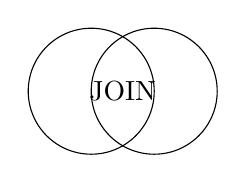
\begin{tikzpicture}
				\draw (0,0) circle (0.8);
				\draw (0.8,0) circle (0.8);
				\node at (0.4,0) {JOIN};
			\end{tikzpicture}
		\end{columns}
	\end{frame}
	
	\begin{frame}{Join Visualization}
		\begin{center}
			\begin{tabular}{|c|c|}
				\hline
				\textbf{Join Type} & \textbf{Result} \\
				\hline
				INNER JOIN & Matching rows only \\
				\hline
				LEFT JOIN & All left + matching right \\
				\hline
				RIGHT JOIN & All right + matching left \\
				\hline
				FULL OUTER JOIN & All rows from both \\
				\hline
				CROSS JOIN & Cartesian product \\
				\hline
			\end{tabular}
		\end{center}
	\end{frame}
	
	\begin{frame}{Lecture 18: Query Optimization}
		\begin{block}{Optimization Techniques}
			\begin{enumerate}
				\item Use appropriate indexes
				\item Filter early (WHERE before JOIN)
				\item Avoid SELECT *
				\item Use EXPLAIN plan
				\item Partition pruning
				\item Limit result sets
			\end{enumerate}
		\end{block}
		\begin{quote}
			Query conversion and optimization go hand in hand
		\end{quote}
	\end{frame}
	
	
	
	
	% ============================================================
	% BANKING: CROSS-DATABASE QUERY STRATEGIES (8 slides)
	% ============================================================
	
	\begin{frame}{The Challenge: Data Spread Across Systems}
		\begin{center}
			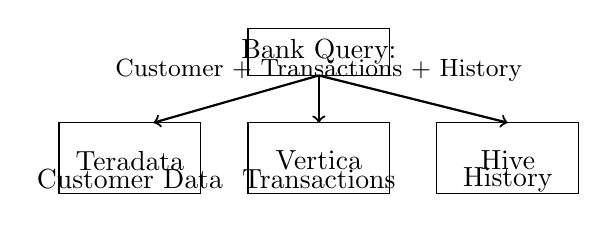
\begin{tikzpicture}[scale=0.6]
				\draw (0,1) rectangle (3,2.5);
				\node at (1.5,1.7) {Teradata};
				\node at (1.5,1.3) {Customer Data};
				
				\draw (4,1) rectangle (7,2.5);
				\node at (5.5,1.7) {Vertica};
				\node at (5.5,1.3) {Transactions};
				
				\draw (8,1) rectangle (11,2.5);
				\node at (9.5,1.7) {Hive};
				\node at (9.5,1.3) {History};
				
				\draw (4,3.5) rectangle (7,4.5);
				\node at (5.5,4) {Bank Query:};
				\node at (5.5,3.6) {\small Customer + Transactions + History};
				
				\draw[->, thick] (5.5,3.5) -- (2,2.5);
				\draw[->, thick] (5.5,3.5) -- (5.5,2.5);
				\draw[->, thick] (5.5,3.5) -- (9.5,2.5);
			\end{tikzpicture}
		\end{center}
		
		\begin{alertblock}{The Problem}
			\begin{itemize}
				\small
				\item Customer data in Teradata
				\item Daily transactions in Vertica
				\item Historical archive in Hive
				\item Query needs data from ALL THREE
			\end{itemize}
		\end{alertblock}
	\end{frame}
	
	
	\begin{frame}{Solution 1: Federation Layer (Toad Data Point)}
		\begin{block}{Cross-Connection Query in Toad}
			Toad allows joining tables from different databases in one query.
		\end{block}
		
		\begin{example}{Toad Cross-Connection Setup}
			\begin{enumerate}
				\small
				\item Create connection to Teradata (Customer DB)
				\item Create connection to Vertica (Transactions DB)
				\item Create connection to Hive (History DB)
				\item Write SQL that references ALL three
			\end{enumerate}
		\end{example}
		
		\begin{center}
			\textcolor{blue}{Prerequisite:} ODBC drivers for ALL databases must be installed
		\end{center}
	\end{frame}
	
	
	\begin{frame}{Complex Bank SQL Query Example}
		\begin{block}{Query: Customer Risk Score with History}
			\small
			\color{blue}
			SELECT c.customer\_id, c.customer\_name, c.credit\_score,\par
			SUM(t.transaction\_amount) as total\_spend,\par
			COUNT(h.transaction\_id) as historical\_txns\par
			FROM Teradata.bank\_db.customers c\par
			LEFT JOIN Vertica.bank\_db.transactions t\par
			ON c.customer\_id = t.customer\_id\par
			AND t.transaction\_date >= '2024-01-01'\par
			LEFT JOIN Hive.archive\_db.historical\_txns h\par
			ON c.customer\_id = h.customer\_id\par
			WHERE c.credit\_score < 650\par
			GROUP BY c.customer\_id, c.customer\_name, c.credit\_score\par
			HAVING SUM(t.transaction\_amount) > 10000
			\color{black}
		\end{block}
		
		\begin{center}
			\textcolor{orange}{Note:} Syntax varies by tool. Toad uses [DB].table format.
		\end{center}
	\end{frame}
	
	
	\begin{frame}{How Banks Actually Handle This (Best Practices)}
		\begin{columns}[T]
			\column{0.48\textwidth}
			\begin{block}{Method 1: ETL to Central EDW}
				\begin{itemize}
					\small
					\item Copy all data to Teradata
					\item Run queries locally
					\item PRO: Simple, fast joins
					\item CON: Data duplication
				\end{itemize}
			\end{block}
			
			\column{0.48\textwidth}
			\begin{block}{Method 2: Federation (Toad)}
				\begin{itemize}
					\small
					\item Query across sources live
					\item No data movement
					\item PRO: Real-time data
					\item CON: Slower performance
				\end{itemize}
			\end{block}
		\end{columns}
		
		\vspace{0.3cm}
		\begin{columns}[T]
			\column{0.48\textwidth}
			\begin{block}{Method 3: Data Lake}
				\begin{itemize}
					\small
					\item Land ALL data in Hive
					\item Use Spark for joins
					\item PRO: Scalable, cheap
					\item CON: Batch only
				\end{itemize}
			\end{block}
			
			\column{0.48\textwidth}
			\begin{block}{Method 4: API Layer}
				\begin{itemize}
					\small
					\item Query each source separately
					\item Join in application code
					\item PRO: Flexible
					\item CON: Complex code
				\end{itemize}
			\end{block}
		\end{columns}
	\end{frame}
	
	
	\begin{frame}{Practical Tips for Complex Cross-Database Queries}
		\begin{block}{Step-by-Step Approach}
			\begin{enumerate}
				\small
				\item Identify source of truth for each data element
				\item Start small - test joins with LIMIT 100 first
				\item Filter early - push WHERE to each source
				\item Use staging tables for frequently joined data
				\item Create views to simplify complex logic
			\end{enumerate}
		\end{block}
		
		\begin{example}{Reaching Data Quickly}
			\begin{itemize}
				\small
				\item Use SELECT TOP or LIMIT for testing
				\item Check EXPLAIN plan before full execution
				\item Create materialized views for common joins
				\item Use batch windows for large historical joins
			\end{itemize}
		\end{example}
		
		\begin{center}
			\textcolor{orange}{Bank's Secret:} Most complex joins run overnight
		\end{center}
	\end{frame}
	
	
	\begin{frame}{Toad Syntax Pattern for Cross-Database Queries}
		\begin{block}{Toad Connection Format}
			\small
			\color{blue}
			Step 1: Create connections in Toad\par
			- Connection1: Teradata (TD)\par
			- Connection2: Vertica (VC)\par
			- Connection3: Hive (HV)\par
			\vspace{0.2cm}
			Step 2: Write query with [Connection].Database.Table\par
			SELECT\par
			\quad TD.customers.cust\_id,\par
			\quad VC.sales.amount,\par
			\quad HV.history.txn\_date\par
			FROM [Teradata].bank\_db.customers TD\par
			LEFT JOIN [Vertica].bank\_db.sales VC\par
			\quad ON TD.cust\_id = VC.cust\_id\par
			LEFT JOIN [Hive].archive\_db.history HV\par
			\quad ON TD.cust\_id = HV.cust\_id\par
			WHERE VC.sales.amount > 1000
			\color{black}
		\end{block}
	\end{frame}
	
	
	\begin{frame}{Bank's Real-World Data Movement Architecture}
		\begin{center}
			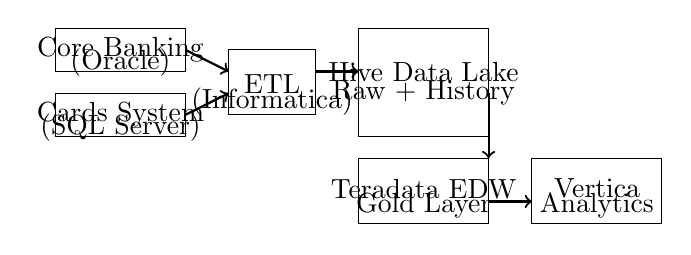
\begin{tikzpicture}[scale=0.55]
				% Source Systems
				\draw (0,2.5) rectangle (3,3.5);
				\node at (1.5,3) {Core Banking};
				\node at (1.5,2.7) {(Oracle)};
				
				\draw (0,1) rectangle (3,2);
				\node at (1.5,1.5) {Cards System};
				\node at (1.5,1.2) {(SQL Server)};
				
				% ETL
				\draw (4,1.5) rectangle (6,3);
				\node at (5,2.2) {ETL};
				\node at (5,1.8) {(Informatica)};
				
				% Data Lake
				\draw (7,1) rectangle (10,3.5);
				\node at (8.5,2.5) {Hive Data Lake};
				\node at (8.5,2) {Raw + History};
				
				% EDW
				\draw (7,-1) rectangle (10,0.5);
				\node at (8.5,-0.2) {Teradata EDW};
				\node at (8.5,-0.6) {Gold Layer};
				
				% Analytics
				\draw (11,-1) rectangle (14,0.5);
				\node at (12.5,-0.2) {Vertica};
				\node at (12.5,-0.6) {Analytics};
				
				% Arrows
				\draw[->, thick] (3,3) -- (4,2.5);
				\draw[->, thick] (3,1.5) -- (4,2);
				\draw[->, thick] (6,2.5) -- (7,2.5);
				\draw[->, thick] (10,2) -- (10,0.5);
				\draw[->, thick] (10,-0.5) -- (11,-0.5);
			\end{tikzpicture}
		\end{center}
		
		\begin{example}{Data Flow}
			Sources to ETL to Hive (Landing) to Teradata (Gold) to Vertica (Analytics)
		\end{example}
	\end{frame}
	
	
	\begin{frame}{Quick Reference: Reaching Data Across Systems}
		\begin{table}
			\small
			\begin{tabular}{|p{0.35\textwidth}|p{0.55\textwidth}|}
				\hline
				\textbf{Scenario} & \textbf{Best Approach} \\
				\hline
				Real-time fraud detection & Query Vertica directly (fastest) \\
				\hline
				End-of-day reporting & Query Teradata (single source of truth) \\
				\hline
				Historical trend analysis & Query Hive (cheap, scalable) \\
				\hline
				Join live plus history & ETL history to Teradata first \\
				\hline
				Ad-hoc analysis across sources & Use Toad Federation \\
				\hline
				Daily batch reports & Materialized view in EDW \\
				\hline
			\end{tabular}
		\end{table}
		
		\begin{alertblock}{Golden Rule}
			Do not join across systems in real-time. Move data to one place first.
		\end{alertblock}
	\end{frame}
	
	
	
	% ============================================================
	% SECTION 6: SAS (4 slides)
	% ============================================================
	\section{SAS - Statistical Analysis}
	
	\begin{frame}{Lecture 19: Intro to SAS}
		\begin{definition}{SAS}
			Statistical Analysis System - Software suite for advanced analytics, business intelligence, and data management.
		\end{definition}
		
		\textbf{SAS Code Example:}
		\begin{center}
			\color{blue}
			PROC PRINT DATA=work.sales;\\
			WHERE region = EAST;\\
			RUN;
			\color{black}
		\end{center}
	\end{frame}
	
	\begin{frame}{Lecture 20: Why SAS}
		\begin{block}{SAS Strengths}
			\begin{itemize}
				\item Industry standard for \textbf{Logistic Regression}
				\item Regulatory compliance (Pharma, Banking)
				\item Robust data cleaning capabilities
				\item Powerful data visualization
				\item Enterprise support
			\end{itemize}
		\end{block}
	\end{frame}
	
	\begin{frame}{SAS Logistic Regression Example}
		\textbf{Logistic Regression Example:}
		\begin{center}
			\color{blue}
			PROC LOGISTIC DATA=credit\_data;\\
			MODEL default = income age debt;\\
			RUN;
			\color{black}
		\end{center}
		
		\begin{example}{Output Includes}
			\begin{itemize}
				\item Coefficient estimates
				\item P-values
				\item Odds ratios
				\item Model fit statistics
			\end{itemize}
		\end{example}
	\end{frame}
	
	\begin{frame}{SAS vs Other Tools}
		\begin{table}
			\small
			\begin{tabular}{|l|c|c|c|}
				\hline
				\textbf{Feature} & \textbf{SAS} & \textbf{Python} & \textbf{R} \\
				\hline
				Regulatory Compliance & High & Low & Low \\
				\hline
				Learning Curve & Steep & Moderate & Steep \\
				\hline
				Cost & High & Free & Free \\
				\hline
				Visualization & Good & Excellent & Good \\
				\hline
				Big Data Support & Moderate & Excellent & Moderate \\
				\hline
			\end{tabular}
		\end{table}
	\end{frame}
	
	
	
	
\begin{frame}{Building ML Model for Wire Transfer Fraud: Where to Get Data}
	\begin{center}
		\textcolor{blue}{\large Where Does Each Data Type Live in the Bank?}
	\end{center}
	
	\begin{table}
		\tiny
		\begin{tabular}{|p{0.28\textwidth}|p{0.22\textwidth}|p{0.22\textwidth}|p{0.22\textwidth}|}
			\hline
			\textbf{Data Needed for Model} & \textbf{Source Database} & \textbf{Why This DB?} & \textbf{Access Method} \\
			\hline
			Transaction Amount, Time, Date & Oracle Exadata & Core OLTP banking ledger & JDBC / ODBC \\
			\hline
			Sender Account History (last 30 days) & Teradata & EDW historical aggregation & SQL \\
			\hline
			Receiver Account History & Teradata & EDW multi-year ledger view & SQL \\
			\hline
			Customer Profile (Age, Location, Tenure) & Teradata & Single source of truth (EDW) & SQL / JDBC \\
			\hline
			Past Fraud Flags (Labels for Training) & Teradata & Audited compliance records & SQL \\
			\hline
			Device IP, Location, Session Data & Vertica & Columnar = fast log analytics & ODBC / JDBC \\
			\hline
			Historical Wire Transfers (5+ years) & Hive & Cheap archival storage & HiveQL / Spark \\
			\hline
			Geographic Risk Scores & Teradata & Central reference data & SQL \\
			\hline
			Counterparty Risk Rating & Oracle Exadata & Risk management system & ODP.NET / SQL \\
			\hline
		\end{tabular}
	\end{table}
	
	\begin{alertblock}{How to Get ALL Data for Modeling}
		\begin{itemize}
			\tiny
			\item \textbf{Step 1:} Extract from Exadata (core transaction) + Teradata (labels + profiles)
			\item \textbf{Step 2:} Join with Vertica (session logs) + Hive (historical archives)
			\item \textbf{Step 3:} Build feature store in Vertica or Spark Feature Store
			\item \textbf{Step 4:} Train model using PySpark or Python (pandas/scikit-learn)
		\end{itemize}
	\end{alertblock}
	
	\begin{center}
		\textcolor{green}{\tiny Final Training Dataset: Exadata (core) + Teradata (labels/profiles) + Vertica/Hive (behavior/history) = Complete Model}
	\end{center}
\end{frame}


\begin{frame}{Loan Default Model: Where Consumer Data Lives in Bank}
	\begin{center}
		\textcolor{blue}{\large Consumer Loan Default Risk - Data Sources}
	\end{center}
	
	\begin{table}
		\tiny
		\begin{tabular}{|p{0.30\textwidth}|p{0.20\textwidth}|p{0.20\textwidth}|p{0.20\textwidth}|}
			\hline
			\textbf{Consumer Data Element} & \textbf{Source DB} & \textbf{Why This DB?} & \textbf{Update Frequency} \\
			\hline
			Credit Score (Bureau Data) & Teradata & System of record for risk & Monthly \\
			\hline
			Income / Employment History & Teradata & Master profile (EDW) & Quarterly \\
			\hline
			Existing Loan Balances & Oracle Exadata & Core loan accounting platform & Real-time / Daily \\
			\hline
			Payment History (12 months) & Teradata & Consolidated ledger view & Daily \\
			\hline
			Late Payment Flags & Oracle Exadata & Loan servicing engine (ACID) & Real-time \\
			\hline
			Debt-to-Income Ratio & Oracle Exadata & Calculated at origination & Static per application \\
			\hline
			Customer Address / City & Teradata & Master record (MDM Hub) & As needed \\
			\hline
			Economic Data (Unemployment by City) & Hive & External batch data staging & Monthly \\
			\hline
			Property Value (Collateral) & Oracle Exadata & Loan origination platform & Yearly / At Appraisal \\
			\hline
			Past Default Labels (Training) & Teradata & Historical risk warehouse & Static \\
			\hline
			Transaction Behavior (Spending patterns) & Vertica & Columnar analytics on card logs & Daily batch / Streaming \\
			\hline
		\end{tabular}
	\end{table}
	
	\begin{block}{Different Data = Different Databases}
		\tiny
		\begin{itemize}
			\item \textcolor{blue}{Teradata} = Customer Master, Historical Payment Views, Credit Scores, Default Labels
			\item \textcolor{green}{Oracle Exadata} = Real-time Balances, Late Flags, DTI, Origination/Collateral Specs
			\item \textcolor{orange}{Vertica} = Card Swipe Logs, Clickstream, Behavioral Analytics Features
			\item \textcolor{red}{Hive} = Macroeconomic Indicators, Cold Historical Backups
		\end{itemize}
	\end{block}
	
	\begin{center}
		\textcolor{orange}{\tiny Model Training: Teradata (Labels/Profiles) + Exadata (Core Balances) + Vertica (Behavior) = Complete Features}
	\end{center}
\end{frame}
	
	% ============================================================
	% SECTION 7: COURSE SUMMARY (4 slides)
	% ============================================================
	\begin{frame}{Course Summary - Part 1}
		\begin{center}
			\Huge Congratulations! \\
			\vspace{0.3cm}
			\Large You've completed the course.
		\end{center}
		
		\begin{block}{What You Learned}
			\begin{itemize}
				\item Data Permissions and Governance
				\item Connection Methods (ODBC, Native, SSO)
				\item Teradata, Oracle, Vertica differences
			\end{itemize}
		\end{block}
	\end{frame}
	
	\begin{frame}{Course Summary - Part 2}
		\begin{block}{Skills Acquired}
			\begin{itemize}
				\item Query Optimization Techniques
				\item SQL to PySpark Conversion
				\item SAS Analytics Basics
				\item Troubleshooting Real Issues
			\end{itemize}
		\end{block}
		
		\begin{center}
			\textcolor{green}{All Learning Objectives Completed!}
		\end{center}
	\end{frame}
	
	\begin{frame}{Key Takeaways}
		\begin{enumerate}
			\item Always check permissions before querying
			\item Choose the right database for your workload
			\item Native drivers are better than ODBC when available
			\item Vertica requires 64-bit ODBC driver
			\item Windows SSO works for Teradata and Oracle only
			\item Always validate AI-generated code
		\end{enumerate}
	\end{frame}
	
	\begin{frame}{Next Steps}
		\begin{block}{Continue Your Learning}
			\begin{itemize}
				\small
				\item Practice with real datasets
				\item Try the exercises in each section
				\item Join the discussion forum
				\item Rate this course on Udemy
			\end{itemize}
		\end{block}
		
		\begin{center}
			\vspace{0.3cm}
			\textbf{Thank you for enrolling!} \\
			\vspace{0.2cm}
			\textcolor{blue}{Keep Learning, Keep Growing!}
		\end{center}
	\end{frame}
	
\end{document}